% REV04 Mon Nov  5 18:12:22 WIB 2018
% START Tue May 22 19:45:45 WIB 2018

% (c) 2018 Rahmat M. Samik-Ibrahim 
% All Rights Reversed --- All Wrongs Ignored.
% This is a free document. 

\newcommand{\revision}{04--05-Nov-2018}
% REV04 Mon Nov  5 18:10:45 WIB 2018
% START Tue May 22 19:45:45 WIB 2018

% (c) 2018 Rahmat M. Samik-Ibrahim 
% All Rights Reversed --- All Wrongs Ignored.
% This is a free document. 

\documentclass[a4paper,12pt,twoside,openright]{memoir}
\newcommand{\authora}{Cicak Bin Kadal}
\newcommand{\authorb}{Dul Latip}
\newcommand{\authorc}{Dr. Pepper's Lonely HCB}
\newcommand{\maintitle}{A Simple \LaTeX\ Book Template}
\newcommand{\subtitle}{with the Memoir Class}
\usepackage{etoolbox}         % break break?
\usepackage{graphicx}         % jpg etc pictures.
\usepackage{hyperref}         % URLs 
\usepackage{lipsum}           % Random text
\usepackage[hyperref]{xcolor} % more hyperref color
\setcounter{tocdepth}{2}      % TOC: 1:section 2:subsection
\makeindex
\listfiles
\hypersetup{
    colorlinks=true,
     citecolor=gray,
     filecolor=gray,      
     linkcolor=gray,
      urlcolor=gray,
}
\newcommand{\gaudeamus}{Gaudeamus igitur. Iuvenes dum sumus. Post iucundam iuventutem. Post molesting senatoras. Noha humus.}
\PassOptionsToPackage{hyphens}{url}
\appto\UrlBreaks{\do\a\do\b\do\c\do\d\do\e\do\f\do\g\do\h\do\i\do\j
\do\k\do\l\do\m\do\n\do\o\do\p\do\q\do\r\do\s\do\t\do\u\do\v\do\w
\do\x\do\y\do\z}


\begin{document}
% REV02 Thu May 24 18:33:02 WIB 2018
% START Tue May 22 19:45:45 WIB 2018

% (c) 2018 Rahmat M. Samik-Ibrahim 
% All Rights Reversed --- All Wrongs Ignored.
% This is a free document. 

\pagenumbering{roman}
\thispagestyle{empty}
\beforepartskip

\newlength{\centeroffset}
\setlength{\centeroffset}{-0.5\oddsidemargin}
\addtolength{\centeroffset}{0.5\evensidemargin}
%\addtolength{\textwidth}{-\centeroffset}
\thispagestyle{empty}
\vspace*{\stretch{1}}
\noindent\hspace*{\centeroffset}\makebox[0pt][l]{\begin{minipage}{\textwidth}
\flushright
{\Huge\bfseries \maintitle}
\noindent\rule[-1ex]{\textwidth}{5pt}\\[2.5ex]
\hfill\emph{\Large \subtitle}
\end{minipage}}

\vspace{\stretch{1}}
\noindent\hspace*{\centeroffset}\makebox[0pt][l]{\begin{minipage}{\textwidth}
\flushright
{\bfseries by 
\authora,\\[1.5ex]
\authorb,\\[1.5ex]
and 
\authorc\\[3ex]} 
Rev. \revision
\end{minipage}}

%\addtolength{\textwidth}{\centeroffset}
\vspace{\stretch{2}}

\pagebreak
\let\cleardoublepage\clearpage

\sloppy
\frontmatter
\begin{small} 
  \noindent Copyright \copyright 2018 \authora, \authorb, and \authorc.
  All rights reversed, all wrongs corrected.

  \lipsum[1]
\end{small}

\chapter{Thank you!}
\noindent%
\lipsum[1]

\newpage \noindent%
The following individuals helped with corrections, suggestions and
material to improve this book:

{\flushleft\small
\authora,
\authorb,
\authorc,
\authora,
\authorb,
\authorc,
\authora,
\authorb,
\authorc,
\authora,
\authorb,
\authorc,
\authora,
\authorb,
\authorc,
\authora,
\authorb,
\authorc,
\authora,
\authorb,
\authorc,
\authora,
\authorb,
\authorc,
\authora,
\authorb,
\authorc.
}

\vspace*{\stretch{1}}

\pagebreak

\chapter{Preface}
\lipsum[1-2]
\vspace{\stretch{1}}

\begin{verse} 
\begin{small} 
\noindent%
\authora{ }(\url{mailto:cbk@cbk.com}), \\
\noindent%
\authorb{ }(\url{https://cbk.vlsm.org/}), \\
\noindent%
and 
\authorc. \\
\noindent%
1600 Pennsylvania Ave NW, Washington, DC 20500,\\
\noindent%
America First.\\
\end{small} 
\end{verse} 
\clearpage

\tableofcontents
\clearpage

\listoffigures
\clearpage

\listoftables
\clearpage

\enlargethispage{\baselineskip}
\mainmatter
\pagenumbering{arabic}


% REV03 Fri May 25 10:23:00 WIB 2018
% START Tue May 22 19:45:45 WIB 2018

% (c) 2018 Rahmat M. Samik-Ibrahim 
% All Rights Reversed --- All Wrongs Ignored.
% This is a free document. 

\chapter{One One One}
\LaTeX{} was originally written by \index{Lamport, Leslie}Leslie Lamport~\cite{lamport94}.
\gaudeamus
\section{Section}
\lipsum[1]
\subsection{SubSection}
\lipsum[1]
See also figure~\ref{document}.
\begin{figure}[h]
\begin{verbatim}
Abcdef ghjijk lmnop qrstu vwxyz.
Abcdef ghjijk lmnop qrstu vwxyz.
Abcdef ghjijk lmnop qrstu vwxyz.
Abcdef ghjijk lmnop qrstu vwxyz.
Abcdef ghjijk lmnop qrstu vwxyz.
\end{verbatim}
\caption[FIG LIST AAAAA]{\gaudeamus}\label{document}
\end{figure}
\subsection{SubSection}
\lipsum[1]
\begin{figure}[h]
\begin{center}
\vspace*{15pt}
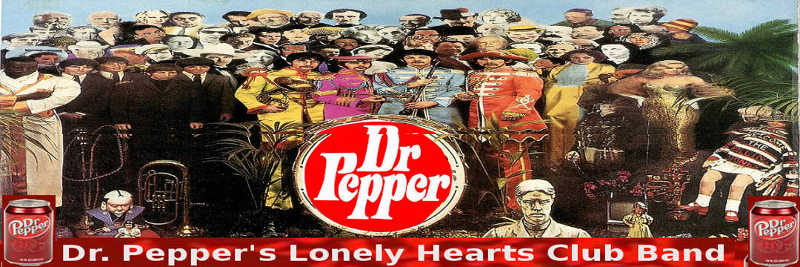
\includegraphics[scale=0.51]{book.jpg}
\end{center}
\caption[FIG LIST BBBBB]{\gaudeamus}\label{fig:figure}
\end{figure}
\lipsum[1]
See also figure~\ref{fig:figure}.
\subsection{SubSection}
\lipsum[1]
\begin{table}[h]
\caption{Table} \label{tab:Table}
\hrule
\begin{description}
\item [\normalfont\texttt{Gaudeamus}] \gaudeamus
\end{description}
\hrule
\end{table}
\lipsum[1]
See also table~\ref{tab:Table}.
This is a long URL: \url{http://texwelt.de/wissen/fragen/5303/%
wiekannichmittikzeinentextamseitenrandvonuntennachobenschreiben}.


% REV02 Thu May 24 18:40:57 WIB 2018
% START Tue May 22 19:45:45 WIB 2018

% (c) 2018 Rahmat M. Samik-Ibrahim 
% All Rights Reversed --- All Wrongs Ignored.
% This is a free document. 

\chapter{Two Two Two}
\lipsum[1-2]


% REV02 Thu May 24 18:40:57 WIB 2018
% START Tue May 22 19:45:45 WIB 2018

% (c) 2018 Rahmat M. Samik-Ibrahim 
% All Rights Reversed --- All Wrongs Ignored.
% This is a free document. 

\chapter{Three Three Three}
\lipsum[1-2]


% REV02 Thu May 24 18:40:57 WIB 2018
% START Tue May 22 19:45:45 WIB 2018

% (c) 2018 Rahmat M. Samik-Ibrahim 
% All Rights Reversed --- All Wrongs Ignored.
% This is a free document. 

\chapter{Four Four Four}
\lipsum[1-2]


% REV02 Thu May 24 20:09:05 WIB 2018
% START Tue May 22 19:45:45 WIB 2018

% (c) 2018 Rahmat M. Samik-Ibrahim 
% All Rights Reversed --- All Wrongs Ignored.
% This is a free document. 

\appendix
\chapter{App App App}
\lipsum[1-5]


% REV04 Mon Nov  5 18:22:04 WIB 2018
% START Tue May 22 19:45:45 WIB 2018

% (c) 2018 Rahmat M. Samik-Ibrahim 
% All Rights Reversed --- All Wrongs Ignored.
% This is a free document. 

\bibliographystyle{plainnat}
\bibliography{rmsbib-list}
\backmatter

%% \begin{thebibliography}{99}
%% \bibitem{lamport94} Leslie Lamport.
%%    \newblock \emph{{\LaTeX:} A Document Preparation System}.
%%    \newblock Addison-Wesley, Reading, Massachusetts, second edition, 1994, ISBN~0-201-52983-1.
%% 
%% \bibitem{oetiker} Tobias Oetiker.
%%    \newblock The Not So Short Introduction to \LaTeX2e.
%%    \newblock Available as \url{https://tobi.oetiker.ch/lshort/lshort.pdf} (Accessed: 2018-05-25).
%% 
%% \end{thebibliography}
%% 

\end{document}

## % Original: bib.tex - A simple article illustrating the use of BibTex
## % Andrew Roberts - June 2003
## 
## \documentclass{article}
## \usepackage{natbib}
## \bibpunct{(}{)}{,}{a}{,}{,}
## \newcommand{\BibTeX}{{\sc Bib}\TeX}
## 
## \begin{document}
## \author{Andrew Roberts}
## \title{A Quick Look at \LaTeX}
## \date{\today}
## \maketitle
## 
## \section{Introduction}
## \LaTeX{} is a typesetting system developed by Leslie
## Lamport \citep{lamport94}.  It builds on foundations created by Donald
## %% ZCZC 
## Knuth's \TeX{} system \citep{knuth79}.  \TeX{} 
## became very popular within
## the scientiic community because it was very good at producing
## mathematical manuscripts.  It was extremely powerful and provided the
## user with exceptional control of the presentation of their documents.
## In the 80s, Lamport began developing \LaTeX, which was designed to add a
## layer of abstraction on top of \TeX{} which allows the user to focus
## more on the document structure, rather than getting too bogged down with
## presentation issues.  \LaTeX{} also added extra functionality through
## auxiliary programs that can generate bibliographies, tables of contents,
## indices, tables, cross-references and figures.
## 
## \section{How to learn more}
## Here are some well established resources to help you learn more about
## this excellent system.
## 
## \begin{itemize}
## 	
## 	\item General \LaTeX{} resources - the excellent \LaTeX{}
##         %% ZCZC Companion \citep{goossens93} is a broad, yet in depth 
##         look at the most important aspects.
## 
##         \item Graphics - take a look at Rahtz's 
##         %% ZCZC	survey \citep{rahtz89} of graphics techniques in \TeX. 
## 
##         \item Bibliographies - the best place to start would be the
##         %% ZCZC	\BibTeX{} documentation by \citet{patashnik88}.
## 
## 	\item Extras - The CTAN 
##         %% ZCZC archives\citep{greenwade93} contain a vast
##         number of supplimentary features, such as packages, macros, styles,
##         etc., that can extend the potential of \LaTeX{} even further.
## 
## \end{itemize}
## 
## \bibliographystyle{plainnat}
## \bibliography{rmsbib-list}
## 
## \end{document}
## 
